\documentclass[12pt, letterpaper]{article}
\usepackage[margin=1in]{geometry}
\usepackage{graphicx}
\usepackage{amsmath}
\usepackage{amssymb}
\usepackage{float}
\usepackage{caption}
\usepackage{subcaption}
\usepackage{booktabs}
\usepackage{hyperref}
\usepackage{fancyhdr}
\usepackage{titlesec}
\usepackage{enumitem}
\usepackage{xcolor}

\setlength{\headheight}{14.5pt}
\addtolength{\topmargin}{-2.5pt}
\pagestyle{fancy}
\fancyhf{}
\rhead{EE 134 -- Homework 2}
\lhead{Kaushik Vada}
\rfoot{Page \thepage}

\titleformat{\section}{\large\bfseries}{Q2.\arabic{section}: }{0em}{}
\titleformat{\subsection}{\normalsize\bfseries}{}{0em}{}

\begin{document}

\begin{center}
    {\LARGE \textbf{Homework 2}} \\[0.5em]
    {\large EE 134 -- Digital IC Design} \\[0.3em]
    {\large Winter 2026} \\[0.3em]
    {\large University of California, Riverside} \\[0.8em]
    {\large Kaushik Vada} \\[0.3em]
    {\large February 18, 2026}
\end{center}

\vspace{1em}

%% ============================================================
%% PART 1: CMOS LOGIC GATES
%% ============================================================
\begin{center}
\rule{0.6\textwidth}{0.4pt}\\[0.3em]
{\Large \textbf{Part 1: CMOS Logic Gates}}\\[0.3em]
\rule{0.6\textwidth}{0.4pt}
\end{center}

%% ----- Q2.1 -----
\section{Complex CMOS Logic Gate}

The complex logic function $Y = \overline{(A \cdot B + E) \cdot (C \cdot D + E)}$ was implemented in CMOS style. The pull-up network (PUN) uses PMOS transistors, and the pull-down network (PDN) uses NMOS transistors, connected as duals of each other. Each input and output port is clearly labeled.

\begin{figure}[H]
    \centering
    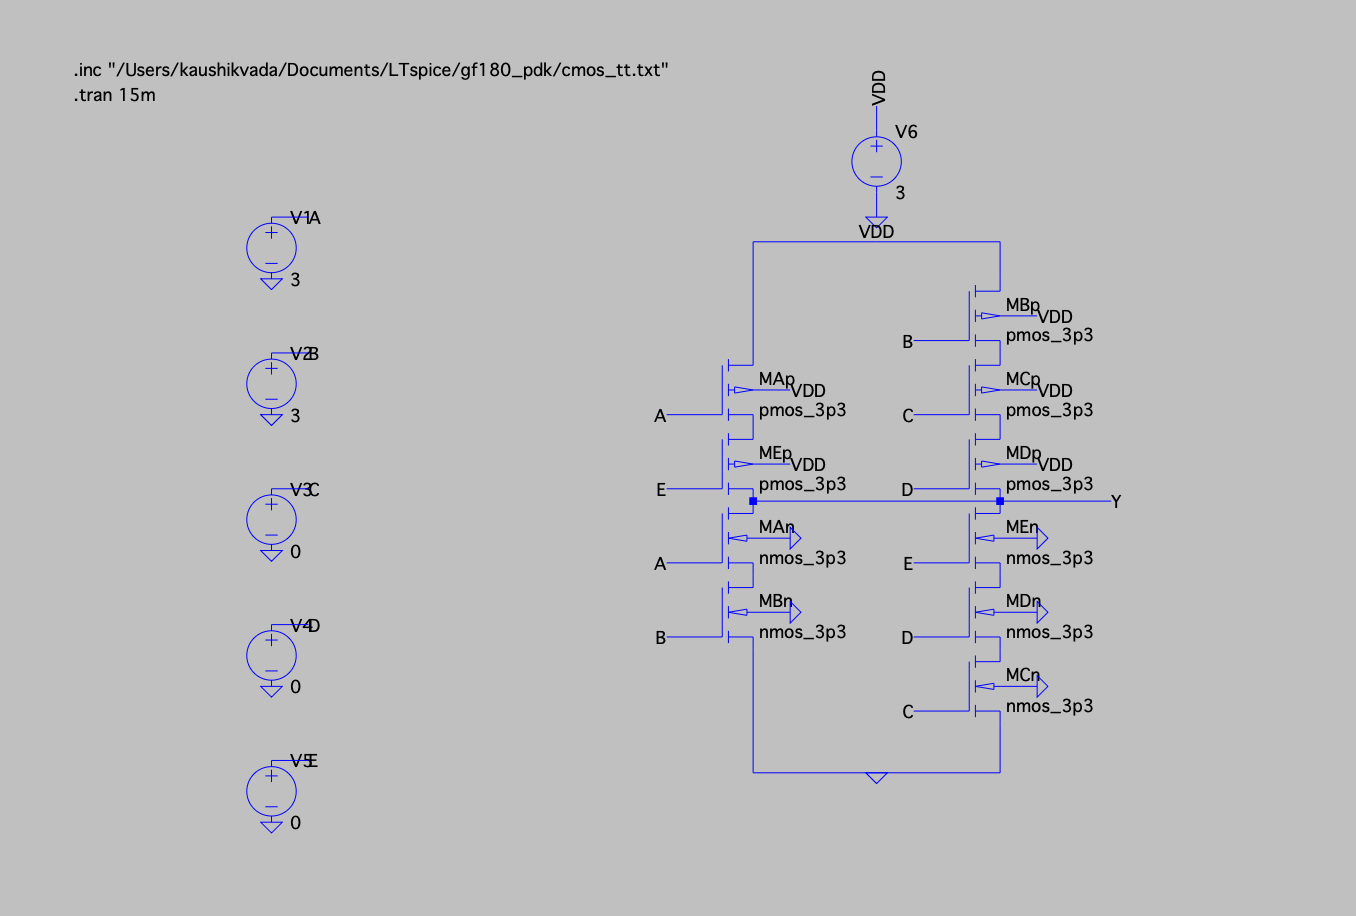
\includegraphics[width=0.85\textwidth]{Q2_1.png}
    \caption{CMOS complex logic gate schematic in LTspice. Inputs A, B, C, D, E and output Y are labeled. The PDN implements the function with series/parallel NMOS networks, while the PUN is the complementary PMOS structure.}
\end{figure}

The PDN consists of two parallel paths to ground: one through the series combination of NMOS transistors A and B in series with E, and another through E in series with the parallel combination of C and D. The PUN is the dual: series PMOS paths where the PDN has parallel, and parallel where the PDN has series.

%% ----- Q2.2 -----
\section{CMOS XOR Gate with Transistor Sizing}

A CMOS XOR gate was designed assuming inverted inputs ($\overline{A}$, $\overline{B}$) are available. The XOR function is:
\[
Y = A \oplus B = A\overline{B} + \overline{A}B
\]

The transistor sizing was determined to match the worst-case equivalent resistance to that of a unit inverter. The unit inverter has PMOS width $W_p = 2$ and NMOS width $W_n = 1$ (all lengths identical).

\begin{figure}[H]
    \centering
    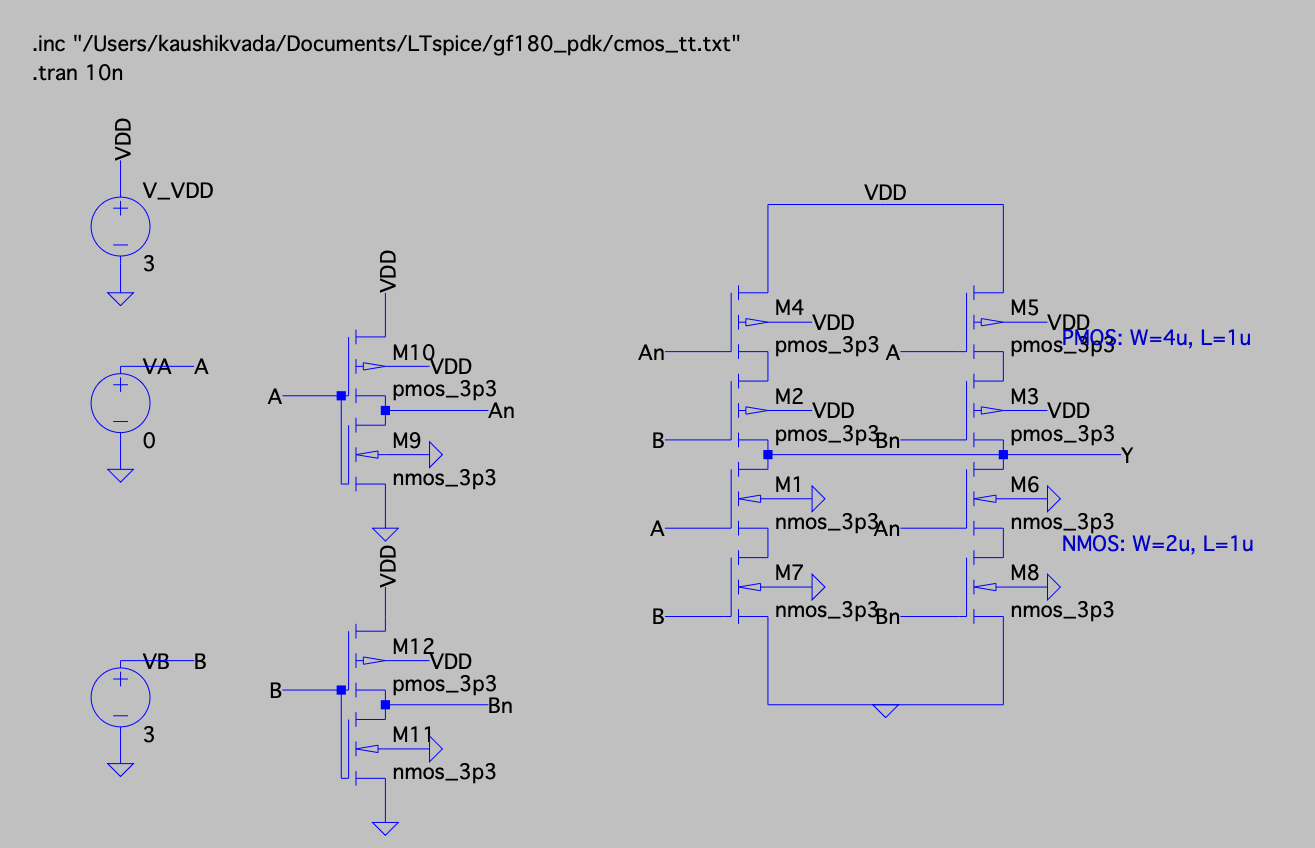
\includegraphics[width=0.85\textwidth]{Q2_2.png}
    \caption{CMOS XOR gate schematic with transistor sizing annotations. PMOS: $W = 4\,\mu$m, $L = 1\,\mu$m. NMOS: $W = 2\,\mu$m, $L = 1\,\mu$m.}
\end{figure}

\subsection{Sizing Analysis}

For the \textbf{pull-down network}: The worst case involves two NMOS transistors in series. To achieve the same equivalent resistance as the unit inverter NMOS ($W_n = 1$), each series NMOS must be sized at $2 \times W_n = 2$.

For the \textbf{pull-up network}: The worst case involves two PMOS transistors in series. To achieve the same equivalent resistance as the unit inverter PMOS ($W_p = 2$), each series PMOS must be sized at $2 \times W_p = 4$.

Therefore: all PMOS transistors are sized at $W = 4\,\mu$m, $L = 1\,\mu$m, and all NMOS transistors are sized at $W = 2\,\mu$m, $L = 1\,\mu$m. No simulation is needed for this question.

%% ----- Q2.3 -----
\section{2-Input CMOS NOR Gate -- Worst-Case Delay}

A 2-input CMOS NOR gate was designed with NMOS sized at $2\,\mu\text{m}/1\,\mu\text{m}$ and PMOS sized at $8\,\mu\text{m}/1\,\mu\text{m}$, driving a $10\,$fF capacitor. Three input transition patterns were tested to determine the worst-case delay.

\begin{figure}[H]
    \centering
    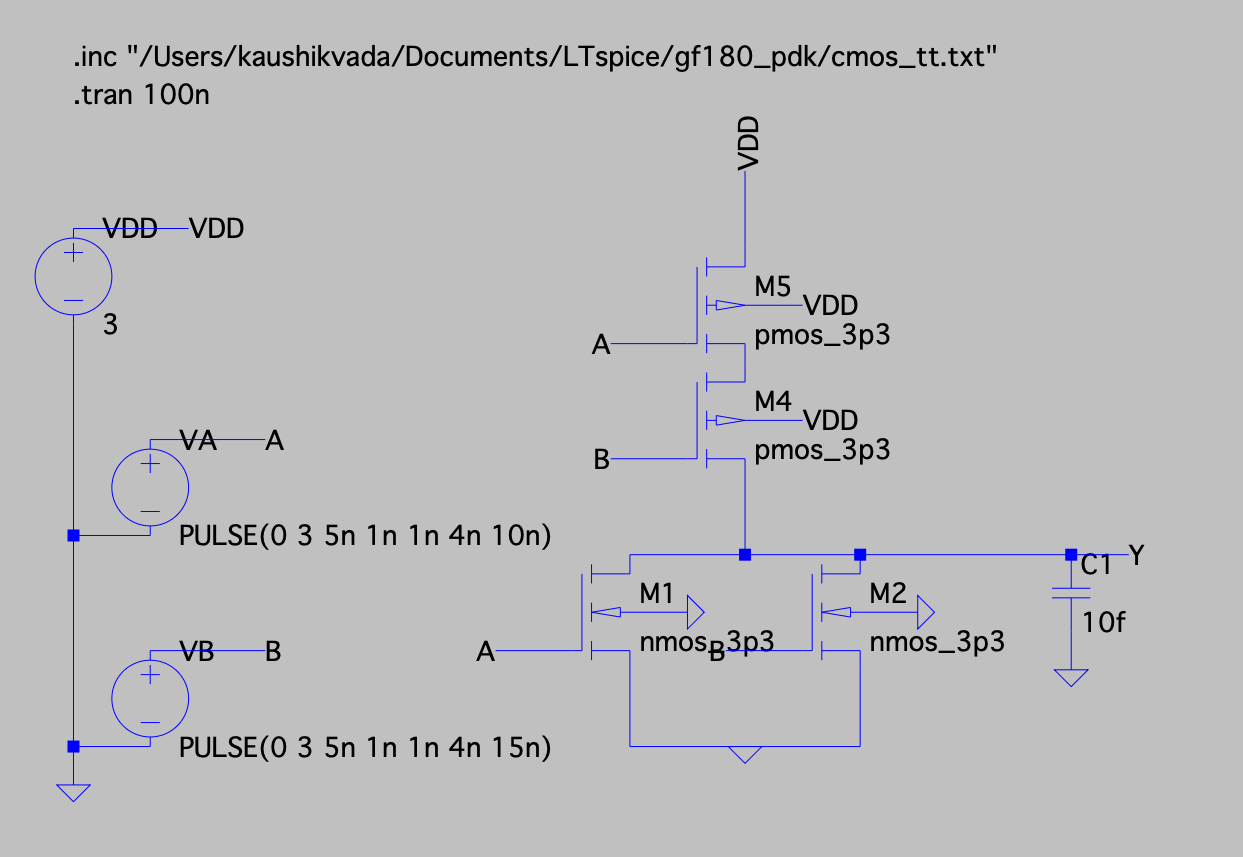
\includegraphics[width=0.75\textwidth]{Question 3/Q2_3.png}
    \caption{NOR gate schematic in LTspice with PULSE inputs and 10\,fF load capacitor.}
\end{figure}

\subsection{Input Pattern 1: Both inputs fall simultaneously (worst-case rising delay)}

Input A has PULSE(0 3 5n 1n 1n 4n 10n) and input B has PULSE(0 3 5n 1n 1n 4n 15n). When both A and B transition high-to-low, the output must rise through two series PMOS transistors.

\begin{figure}[H]
    \centering
    \begin{subfigure}[b]{0.62\textwidth}
        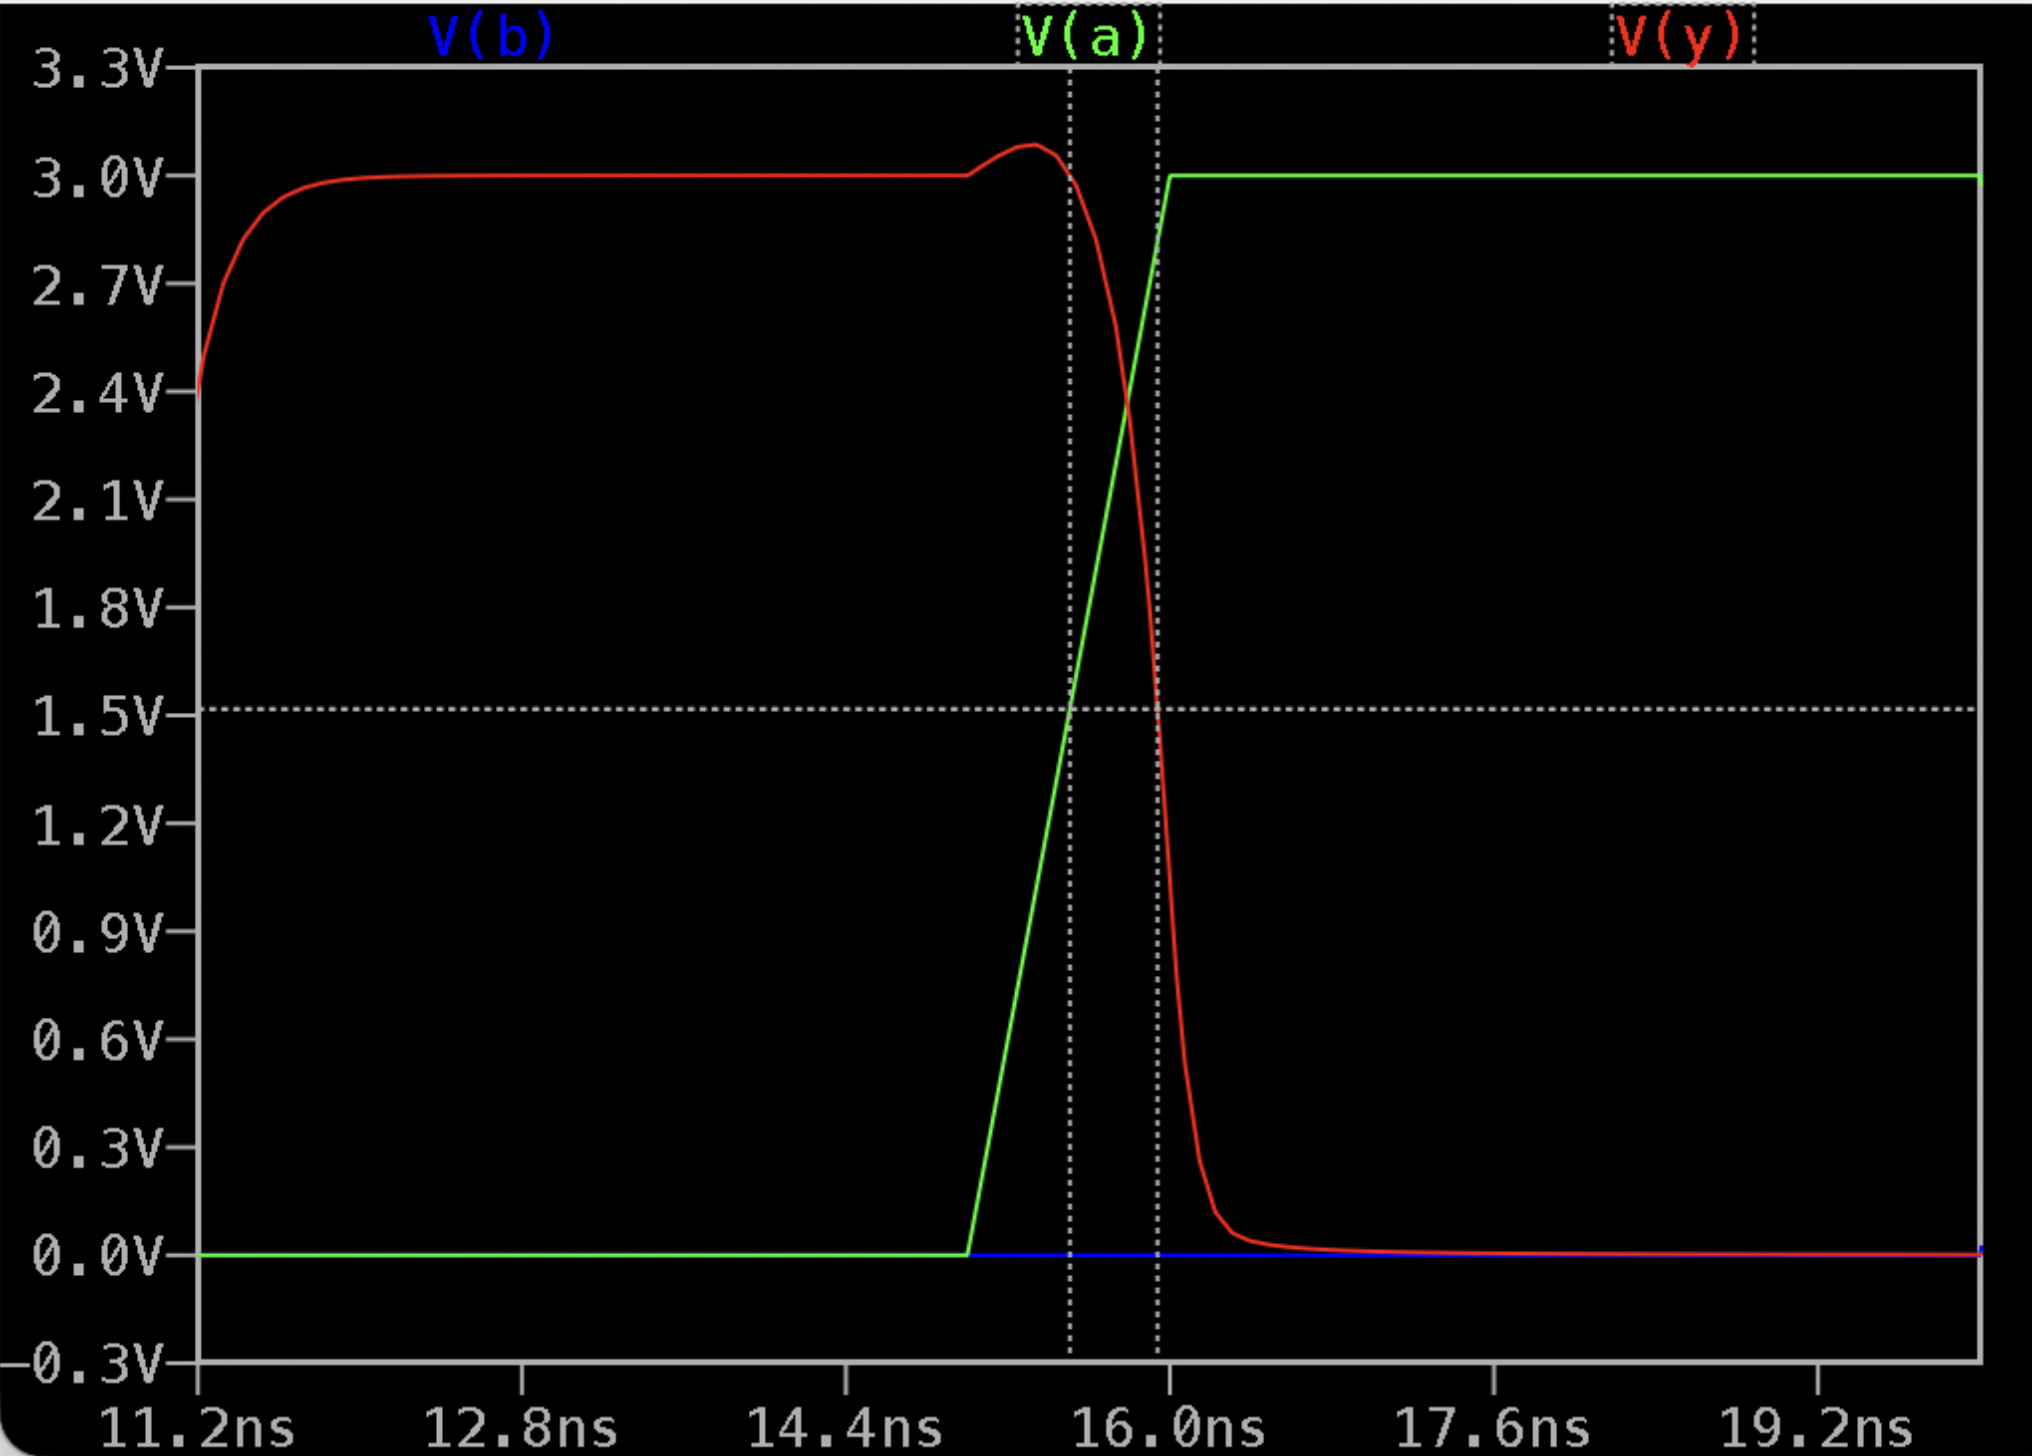
\includegraphics[width=\textwidth]{Question 3/Q2_3(Graph1).png}
        \caption{Waveform: V(a), V(b), V(y)}
    \end{subfigure}
    \hfill
    \begin{subfigure}[b]{0.35\textwidth}
        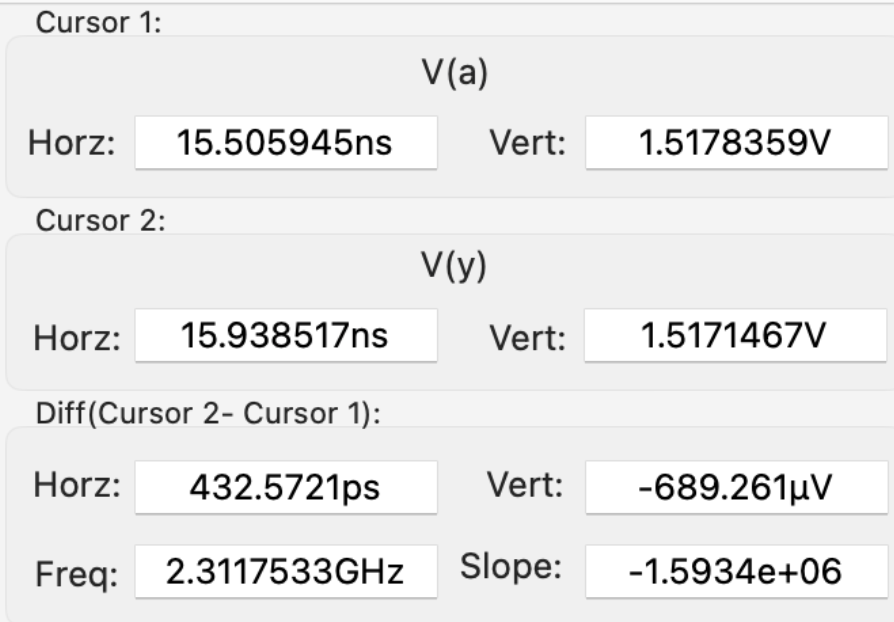
\includegraphics[width=\textwidth]{Question 3/Q2_3(coord1).png}
        \caption{Cursor measurement}
    \end{subfigure}
    \caption{Pattern 1 -- Both inputs fall. Measured delay: $\mathbf{432.6\,\textbf{ps}}$ (from input midpoint at 15.506\,ns to output midpoint at 15.939\,ns).}
\end{figure}

\subsection{Input Pattern 2: One input falls while other stays low (rising delay)}

\begin{figure}[H]
    \centering
    \begin{subfigure}[b]{0.55\textwidth}
        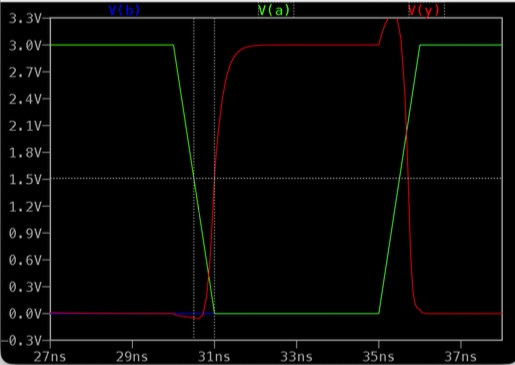
\includegraphics[width=\textwidth]{Question 3/Q2_3(Graph2).png}
        \caption{Waveform}
    \end{subfigure}
    \hfill
    \begin{subfigure}[b]{0.42\textwidth}
        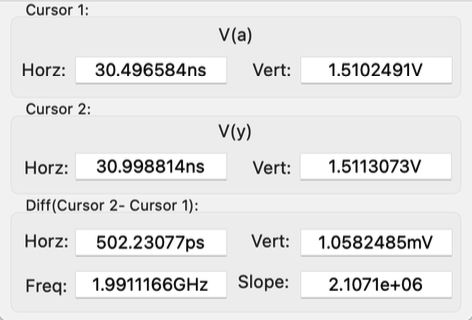
\includegraphics[width=\textwidth]{Question 3/Q2_3(coord2).png}
        \caption{Cursor measurement}
    \end{subfigure}
    \caption{Pattern 2 -- One input falls, other already low. Measured delay: $\mathbf{502.2\,\textbf{ps}}$.}
\end{figure}

\subsection{Input Pattern 3: One input rises while other stays low (falling delay)}

\begin{figure}[H]
    \centering
    \begin{subfigure}[b]{0.55\textwidth}
        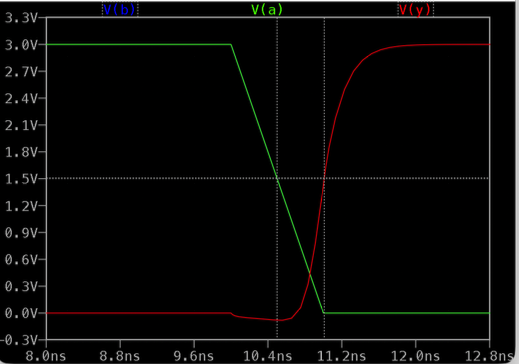
\includegraphics[width=\textwidth]{Question 3/Q2_3(Graph3).png}
        \caption{Waveform}
    \end{subfigure}
    \hfill
    \begin{subfigure}[b]{0.42\textwidth}
        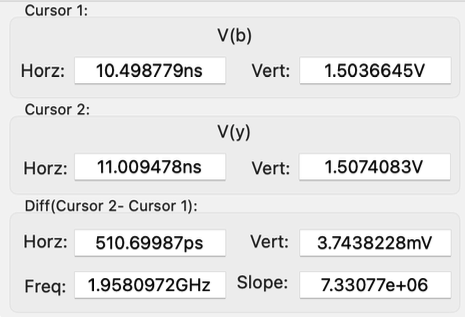
\includegraphics[width=\textwidth]{Question 3/Q2_3(coord3).png}
        \caption{Cursor measurement}
    \end{subfigure}
    \caption{Pattern 3 -- One input rises, other stays low. Measured delay: $\mathbf{510.7\,\textbf{ps}}$.}
\end{figure}

\subsection{Conclusion}

The worst-case delay is \textbf{510.7\,ps}, occurring when a single input transitions low-to-high while the other input remains low (Pattern 3, falling output). This is the worst-case pull-down scenario because only one NMOS is switching and the output must discharge through the parallel NMOS path. The worst-case rising delay (502.2\,ps, Pattern 2) is slightly smaller, as only one series PMOS needs to turn on while the other is already conducting.

\newpage

%% ----- Q2.4 -----
\section{Switching Power Estimation of the NOR Gate}

Using the same NOR gate circuit from Q2.3, the switching power was measured over two different time durations.

\subsection{1000\,ns Transient Simulation}

\begin{figure}[H]
    \centering
    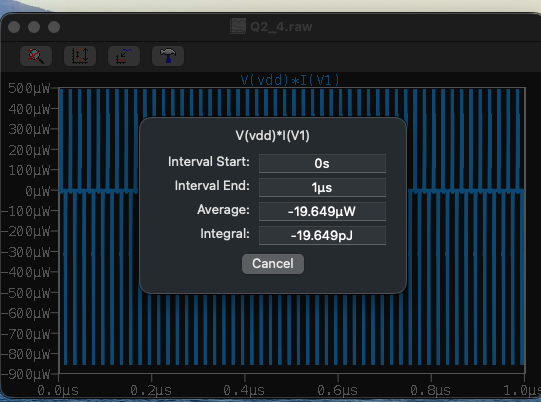
\includegraphics[width=0.65\textwidth]{Question 4/Graph 1.png}
    \caption{Power measurement ($V_{DD} \times I_{V1}$) over 1000\,ns. Average power: $|{-19.649\,\mu\text{W}}| = 19.649\,\mu$W. Energy (integral): $19.649\,$pJ.}
\end{figure}

\subsection{2000\,ns Transient Simulation}

\begin{figure}[H]
    \centering
    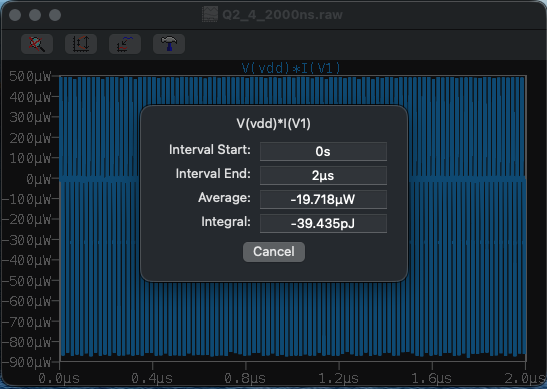
\includegraphics[width=0.65\textwidth]{Question 4/Graph 2.png}
    \caption{Power measurement over 2000\,ns. Average power: $|{-19.718\,\mu\text{W}}| = 19.718\,\mu$W. Energy (integral): $39.435\,$pJ.}
\end{figure}

\subsection{Results Summary}

\begin{table}[H]
\centering
\begin{tabular}{lcc}
\toprule
\textbf{Parameter} & \textbf{1000\,ns} & \textbf{2000\,ns} \\
\midrule
Average Power & 19.649\,$\mu$W & 19.718\,$\mu$W \\
Energy (Integral) & 19.649\,pJ & 39.435\,pJ \\
\bottomrule
\end{tabular}
\caption{Power and energy comparison across simulation durations.}
\end{table}

\subsection{Discussion}

The \textbf{average power stays mostly constant} across time ($\approx 19.65$--$19.72\,\mu$W), while the \textbf{energy increases proportionally} with simulation duration (approximately doubling from 19.6\,pJ to 39.4\,pJ when the time doubles).

This is expected because the switching activity (frequency and pattern) remains the same, so the rate of energy consumption (power) is constant. Energy, being the time integral of power ($E = P \cdot t$), scales linearly with the simulation duration. The switching power is determined by $P_{sw} = \alpha C_L V_{DD}^2 f$, where $\alpha$ is the activity factor, $C_L$ is the load capacitance, and $f$ is the switching frequency -- all of which are constant regardless of simulation length.

\newpage

%% ============================================================
%% PART 2: OTHER LOGIC FAMILIES
%% ============================================================
\begin{center}
\rule{0.6\textwidth}{0.4pt}\\[0.3em]
{\Large \textbf{Part 2: Other Logic Families}}\\[0.3em]
\rule{0.6\textwidth}{0.4pt}
\end{center}

%% ----- Q2.5 -----
\section{NMOS Pass Transistor -- Threshold Voltage Estimation}

An NMOS pass transistor ($2\,\mu\text{m}/1\,\mu\text{m}$) was used to estimate the threshold voltage drop. A DC gate voltage of 3\,V was applied, and the drain was driven by PULSE(0 3 10n 1n 1n 18n 40n). The source drives a 1\,fF load capacitor.

\begin{figure}[H]
    \centering
    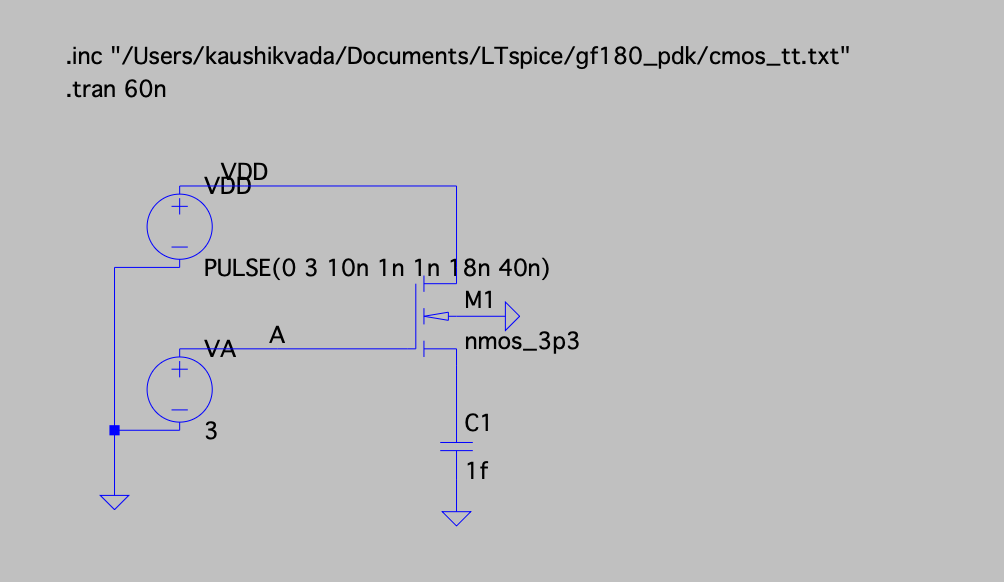
\includegraphics[width=0.65\textwidth]{Question 5/2026-02-18_21-55-22.png}
    \caption{NMOS pass transistor schematic with 3\,V gate bias, pulse drain input, and 1\,fF load.}
\end{figure}

\begin{figure}[H]
    \centering
    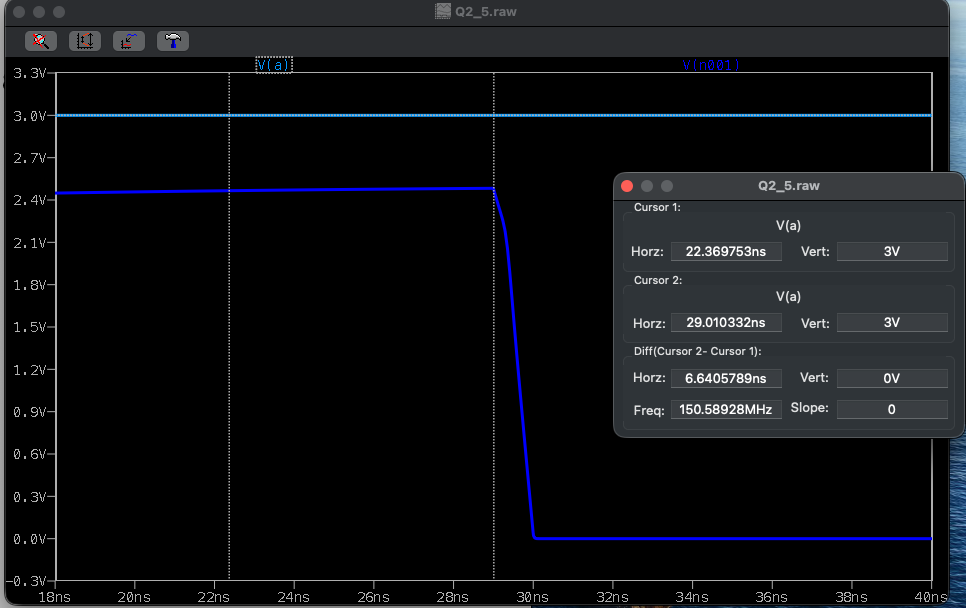
\includegraphics[width=0.75\textwidth]{Question 5/2026-02-18_22-03-43.png}
    \caption{Waveform showing V(a) (input at drain, blue line at $\sim$3\,V) and V(n001) (output at source, cyan). The output settles to approximately 2.4\,V at steady state.}
\end{figure}

\subsection{Result}

The ideal input voltage is 3\,V. The steady-state output voltage is approximately 2.4\,V. The difference gives:
\[
V_{th,n} \approx 3\,\text{V} - 2.4\,\text{V} = \mathbf{0.6\,\textbf{V}}
\]

This $V_{th}$ drop occurs because as the NMOS source voltage rises, $V_{GS}$ decreases. When $V_{GS}$ drops below $V_{th}$, the transistor turns off and can no longer pass a full logic high. The NMOS pass transistor therefore passes a degraded high voltage of $V_{DD} - V_{th}$.

\newpage

%% ----- Q2.6 -----
\section{PMOS Pass Transistor -- Threshold Voltage Estimation}

A PMOS pass transistor ($4\,\mu\text{m}/1\,\mu\text{m}$) was tested. The gate is driven by a pulse, and the source is connected to ground (0\,V). The output voltage is compared with GND.

\begin{figure}[H]
    \centering
    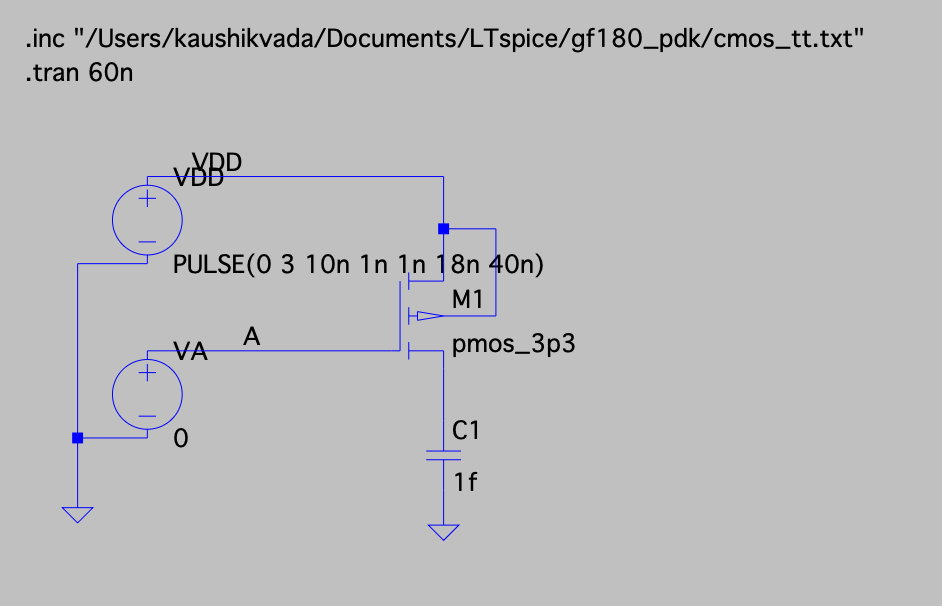
\includegraphics[width=0.6\textwidth]{Question 6/2026-02-18_22-10-52.png}
    \caption{PMOS pass transistor schematic with pulse gate input and 1\,fF load.}
\end{figure}

\begin{figure}[H]
    \centering
    \begin{subfigure}[b]{0.58\textwidth}
        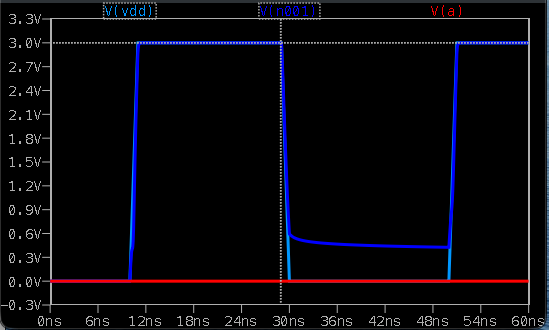
\includegraphics[width=\textwidth]{Question 6/2026-02-18_22-10-58.png}
        \caption{Waveform showing V(vdd) pulse, V(n001) output, and V(a) gate.}
    \end{subfigure}
    \hfill
    \begin{subfigure}[b]{0.38\textwidth}
        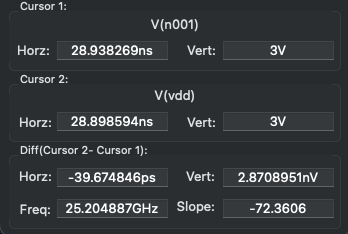
\includegraphics[width=\textwidth]{Question 6/2026-02-18_22-11-02.png}
        \caption{Cursor measurement.}
    \end{subfigure}
    \caption{PMOS pass transistor waveforms. The output settles to approximately 0.4\,V when trying to pass a logic low.}
\end{figure}

\subsection{Result}

The ideal output voltage should match GND at 0\,V. The steady-state output is approximately 0.4\,V. The difference gives:
\[
|V_{th,p}| \approx 0.4\,\text{V} - 0\,\text{V} = \mathbf{0.4\,\textbf{V}}
\]

The PMOS pass transistor passes a strong high (0\,V is a strong low for PMOS) but cannot pass a strong low. The output voltage is degraded by $|V_{th,p}|$, settling at approximately $|V_{th,p}|$ above ground.

\newpage

%% ----- Q2.7 -----
\section{2:1 Multiplexer -- CMOS Gates vs. Transmission Gates}

Two versions of a 2:1 multiplexer ($F = S \cdot A + \overline{S} \cdot B$) were designed. NMOS: $2\,\mu\text{m}/1\,\mu\text{m}$, PMOS: $4\,\mu\text{m}/1\,\mu\text{m}$.

\subsection{Version 1: Standard CMOS Gates}

\begin{figure}[H]
    \centering
    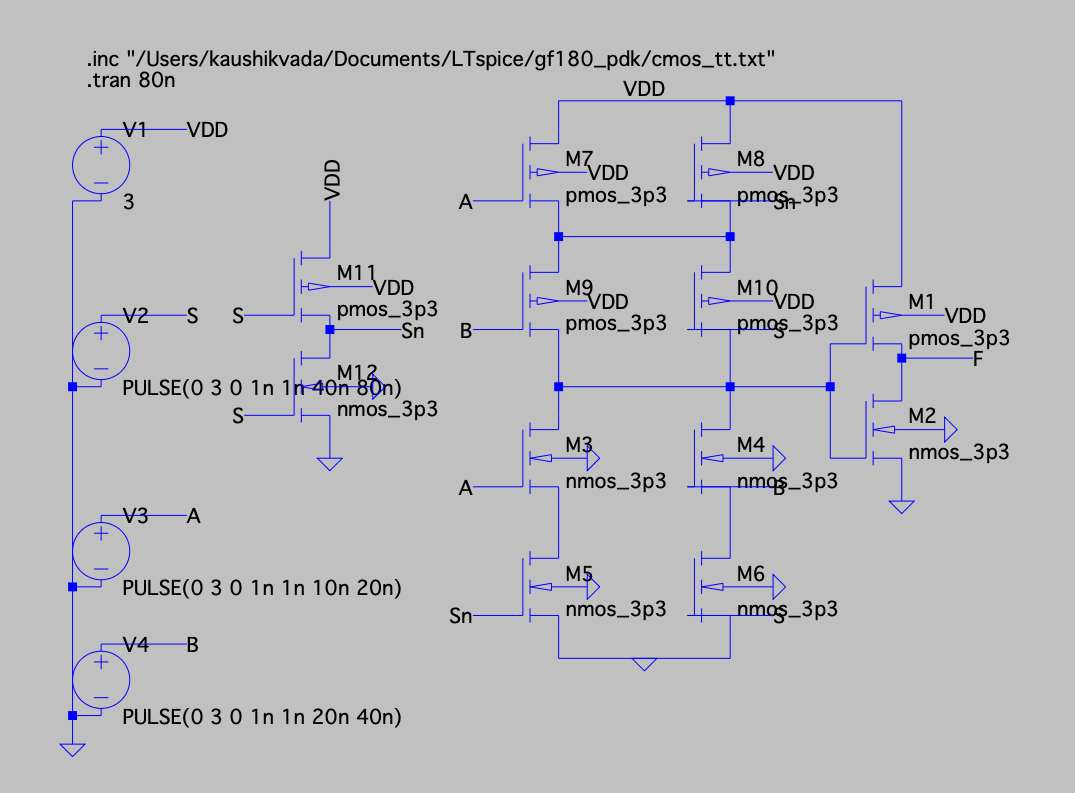
\includegraphics[width=0.85\textwidth]{Question 7/2026-02-18_22-20-56.png}
    \caption{CMOS gate-based 2:1 MUX schematic. Implemented as two AND gates feeding an OR gate, with an inverter to generate $\overline{S}$.}
\end{figure}

\begin{figure}[H]
    \centering
    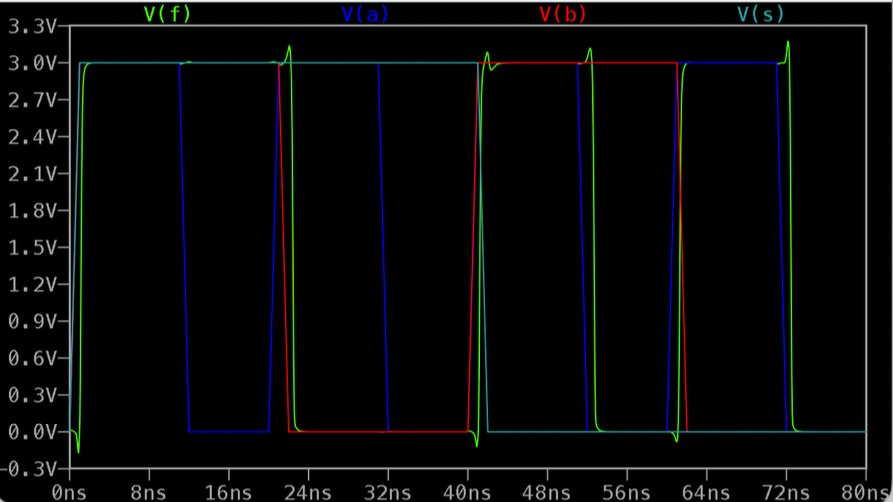
\includegraphics[width=0.75\textwidth]{Question 7/2026-02-18_22-21-39.png}
    \caption{Full transient waveforms: V(f) output, V(a), V(b) data inputs, V(s) select signal.}
\end{figure}

\begin{figure}[H]
    \centering
    \begin{subfigure}[b]{0.48\textwidth}
        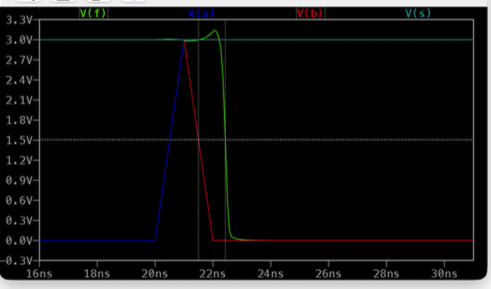
\includegraphics[width=\textwidth]{Question 7/2026-02-18_22-31-09.png}
        \caption{Zoomed rising transition}
    \end{subfigure}
    \hfill
    \begin{subfigure}[b]{0.48\textwidth}
        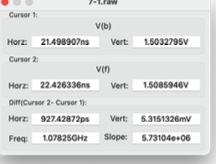
\includegraphics[width=\textwidth]{Question 7/2026-02-18_22-31-21.png}
        \caption{Rising delay: 927.4\,ps}
    \end{subfigure}
    \caption{CMOS MUX worst-case rising delay measurement.}
\end{figure}

\begin{figure}[H]
    \centering
    \begin{subfigure}[b]{0.48\textwidth}
        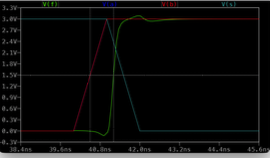
\includegraphics[width=\textwidth]{Question 7/2026-02-18_22-31-41.png}
        \caption{Zoomed falling transition}
    \end{subfigure}
    \hfill
    \begin{subfigure}[b]{0.48\textwidth}
        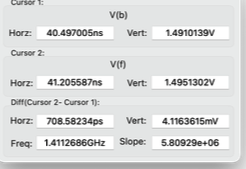
\includegraphics[width=\textwidth]{Question 7/2026-02-18_22-31-46.png}
        \caption{Falling delay: 708.6\,ps}
    \end{subfigure}
    \caption{CMOS MUX worst-case falling delay measurement.}
\end{figure}

\textbf{CMOS MUX worst-case latency: 927.4\,ps} (rising transition).

\subsection{Version 2: Transmission Gate MUX}

\begin{figure}[H]
    \centering
    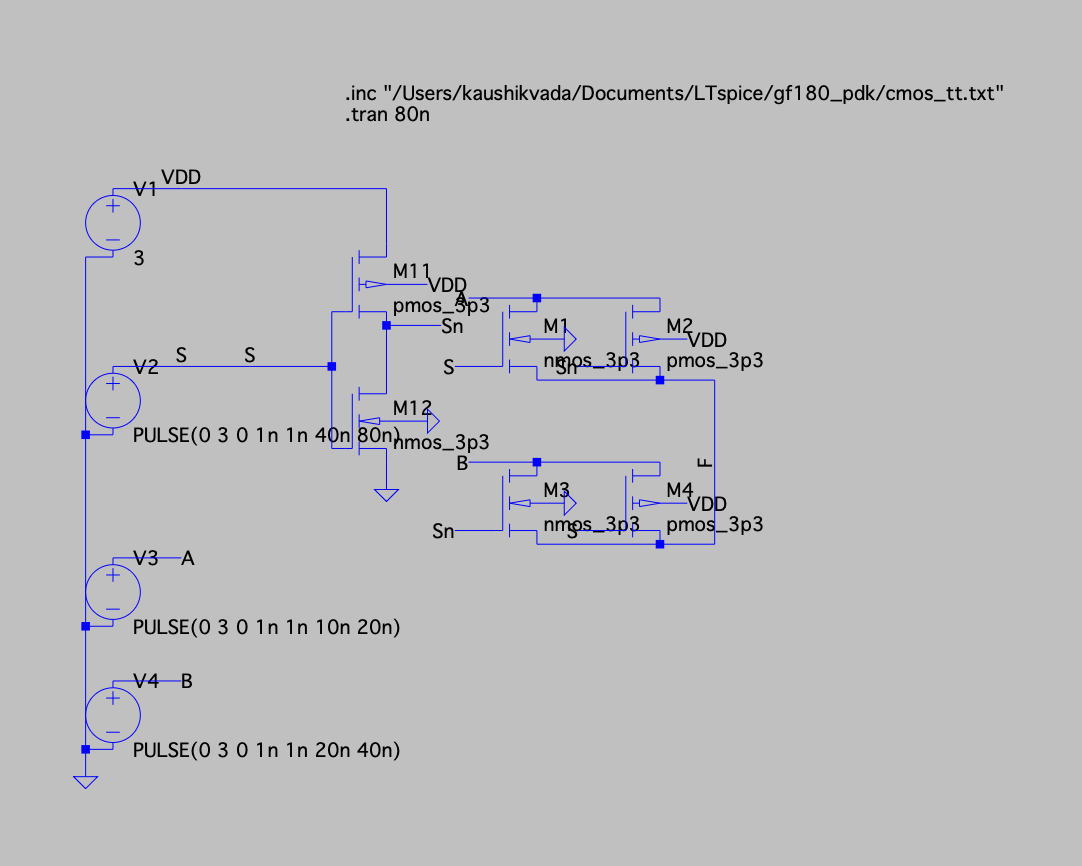
\includegraphics[width=0.75\textwidth]{Question 7/2026-02-18_22-51-09.png}
    \caption{Transmission gate-based 2:1 MUX schematic. Two transmission gates select between inputs A and B based on S and $\overline{S}$.}
\end{figure}

\begin{figure}[H]
    \centering
    \begin{subfigure}[b]{0.48\textwidth}
        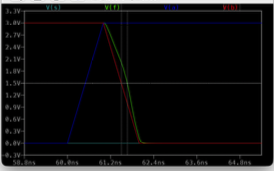
\includegraphics[width=\textwidth]{Question 7/2026-02-18_22-52-05.png}
        \caption{Zoomed transition}
    \end{subfigure}
    \hfill
    \begin{subfigure}[b]{0.48\textwidth}
        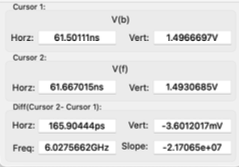
\includegraphics[width=\textwidth]{Question 7/2026-02-18_22-52-13.png}
        \caption{Delay: 165.9\,ps}
    \end{subfigure}
    \caption{Transmission gate MUX worst-case delay measurement.}
\end{figure}

\textbf{Transmission gate MUX worst-case latency: 165.9\,ps}.

\subsection{Comparison}

\begin{table}[H]
\centering
\begin{tabular}{lc}
\toprule
\textbf{Design} & \textbf{Worst-Case Latency} \\
\midrule
CMOS Gate MUX & 927.4\,ps \\
Transmission Gate MUX & 165.9\,ps \\
\bottomrule
\end{tabular}
\caption{Latency comparison of the two MUX designs.}
\end{table}

The transmission gate MUX is significantly faster ($\sim$5.6$\times$) because the signal passes through only one transmission gate (a single stage), whereas the CMOS implementation requires multiple logic stages (inverter + AND-OR), each adding propagation delay.

\newpage

%% ----- Q2.8 -----
\section{Power Comparison of MUX Designs}

The average power consumption of both MUX designs from Q2.7 was measured over 1000\,ns.

\begin{figure}[H]
    \centering
    \begin{subfigure}[b]{0.48\textwidth}
        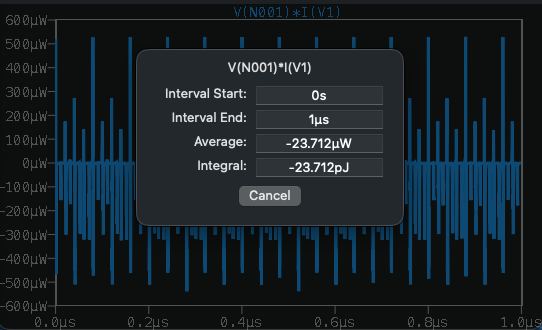
\includegraphics[width=\textwidth]{Question 8/2026-02-18_23-06-15.png}
        \caption{CMOS gate MUX: $|{-23.712\,\mu\text{W}}| = 23.712\,\mu$W}
    \end{subfigure}
    \hfill
    \begin{subfigure}[b]{0.48\textwidth}
        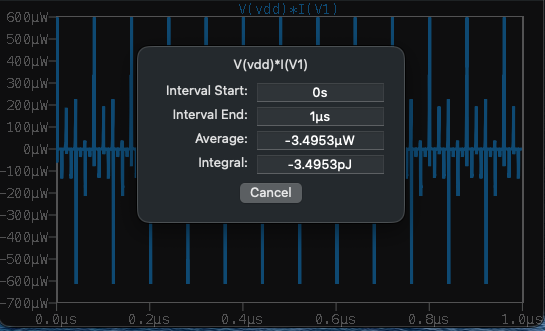
\includegraphics[width=\textwidth]{Question 8/2026-02-18_23-07-25.png}
        \caption{TG MUX: $|{-3.4953\,\mu\text{W}}| = 3.495\,\mu$W}
    \end{subfigure}
    \caption{Average power consumption comparison over 1000\,ns.}
\end{figure}

\begin{table}[H]
\centering
\begin{tabular}{lcc}
\toprule
\textbf{Design} & \textbf{Average Power} & \textbf{Energy (1\,$\mu$s)} \\
\midrule
CMOS Gate MUX & 23.712\,$\mu$W & 23.712\,pJ \\
Transmission Gate MUX & 3.495\,$\mu$W & 3.495\,pJ \\
\bottomrule
\end{tabular}
\caption{Power and energy comparison of MUX implementations.}
\end{table}

\subsection{Discussion}

The CMOS gate-based MUX consumes approximately $6.8\times$ more power than the transmission gate MUX. This is because the CMOS implementation uses many more transistors (inverter, AND gates, OR gate), and each internal node that switches contributes to dynamic power dissipation ($P = \alpha C V_{DD}^2 f$). Additionally, the CMOS gates have short-circuit current during transitions when both PMOS and NMOS are momentarily on. The transmission gate MUX has far fewer transistors, fewer internal switching nodes, and minimal short-circuit current, resulting in significantly lower power consumption.

\newpage

%% ----- Q2.9 -----
\section{Dynamic Logic NAND Gate}

A 2-input NAND gate was designed using dynamic logic style with a footer evaluation transistor. NMOS: $3\,\mu\text{m}/1\,\mu\text{m}$, PMOS (precharge): $1\,\mu\text{m}/1\,\mu\text{m}$. Both input data and clock use PULSE(0 3 5n 1n 1n 8n 20n).

\begin{figure}[H]
    \centering
    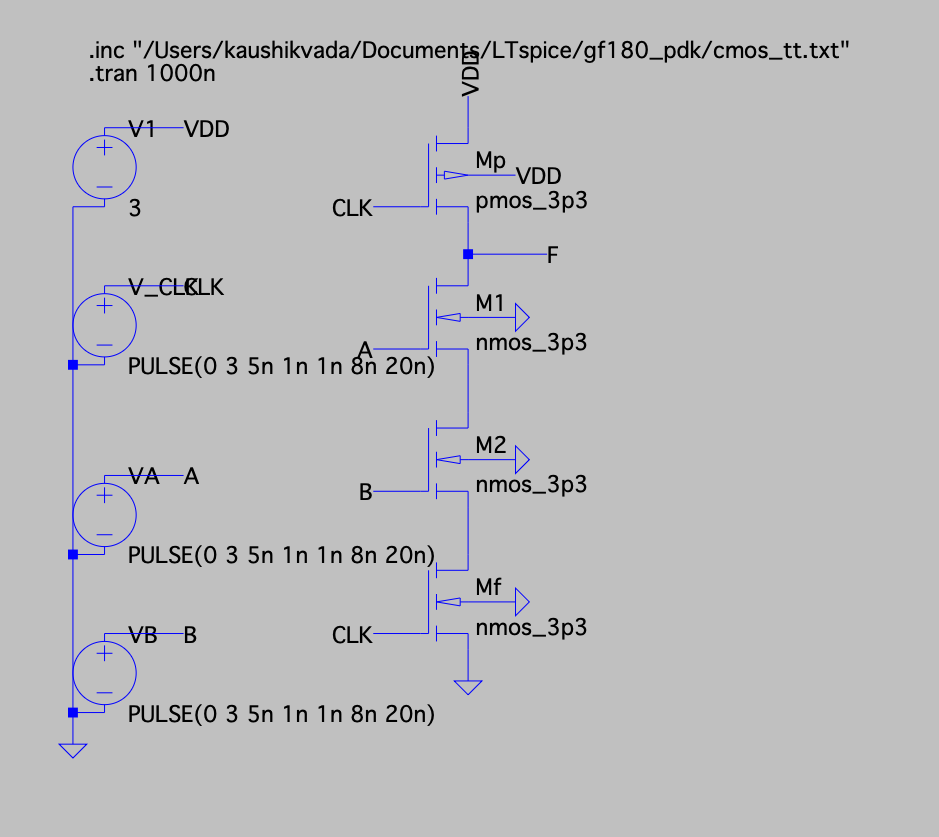
\includegraphics[width=0.65\textwidth]{Question 9/2026-02-18_23-08-21.png}
    \caption{Dynamic NAND gate schematic. PMOS precharge transistor (Mp) controlled by CLK, two series NMOS (M1, M2) for inputs A and B, and footer NMOS (Mf) controlled by CLK for evaluation.}
\end{figure}

\begin{figure}[H]
    \centering
    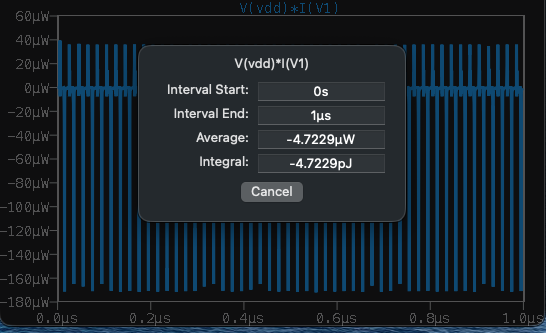
\includegraphics[width=0.65\textwidth]{Question 9/2026-02-18_23-08-16.png}
    \caption{Power measurement over 1000\,ns. Average power: $|{-4.7229\,\mu\text{W}}| = 4.723\,\mu$W. Energy: 4.723\,pJ.}
\end{figure}

The average power consumption of the dynamic NAND gate is \textbf{4.723\,$\mu$W} over 1000\,ns.

\newpage

%% ----- Q2.10 -----
\section{Dynamic vs.\ CMOS NAND Gate -- Speed Comparison}

The worst-case delay of the dynamic NAND gate from Q2.9 was compared with a standard CMOS NAND gate (NMOS: $2\,\mu\text{m}/1\,\mu\text{m}$, PMOS: $2\,\mu\text{m}/1\,\mu\text{m}$).

\subsection{Dynamic NAND Gate Worst-Case Delay}

The worst-case switching pattern for a dynamic NAND gate is when both inputs A and B are high during the evaluation phase (CLK goes high). This causes the precharged output node to discharge through three series NMOS transistors (M1, M2, and the footer Mf).

\begin{figure}[H]
    \centering
    \begin{subfigure}[b]{0.55\textwidth}
        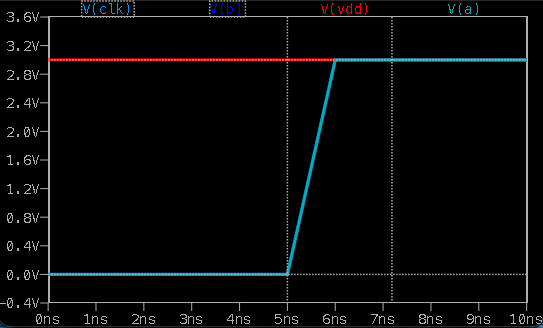
\includegraphics[width=\textwidth]{Question 10/2026-02-18_23-12-25.png}
        \caption{Waveform showing precharge and evaluation.}
    \end{subfigure}
    \hfill
    \begin{subfigure}[b]{0.42\textwidth}
        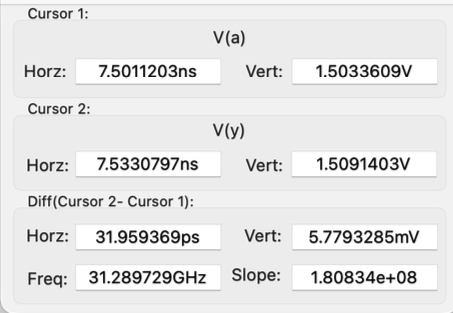
\includegraphics[width=\textwidth]{Question 10/2026-02-18_23-12-08.png}
        \caption{Delay: 32.0\,ps}
    \end{subfigure}
    \caption{Dynamic NAND worst-case delay measurement. The delay from CLK midpoint to output midpoint is approximately \textbf{32.0\,ps}.}
\end{figure}

\subsection{CMOS NAND Gate Worst-Case Delay}

\begin{figure}[H]
    \centering
    \begin{subfigure}[b]{0.55\textwidth}
        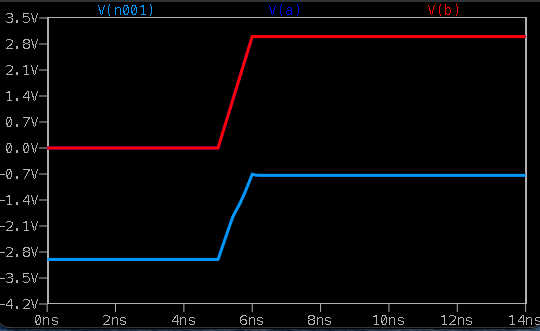
\includegraphics[width=\textwidth]{Question 10/2026-02-18_23-14-33.png}
        \caption{CMOS NAND waveform.}
    \end{subfigure}
    \hfill
    \begin{subfigure}[b]{0.42\textwidth}
        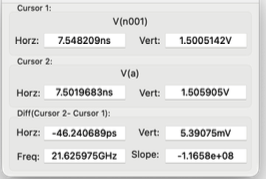
\includegraphics[width=\textwidth]{Question 10/2026-02-18_23-14-42.png}
        \caption{Delay: 46.2\,ps}
    \end{subfigure}
    \caption{CMOS NAND worst-case delay measurement. The delay is approximately \textbf{46.2\,ps}.}
\end{figure}

\subsection{Comparison and Discussion}

\begin{table}[H]
\centering
\begin{tabular}{lc}
\toprule
\textbf{Design} & \textbf{Worst-Case Delay} \\
\midrule
Dynamic NAND (footer) & $\sim$32.0\,ps \\
CMOS NAND & $\sim$46.2\,ps \\
\bottomrule
\end{tabular}
\caption{Delay comparison between dynamic and CMOS NAND gates.}
\end{table}

The dynamic NAND gate is faster than the CMOS NAND gate ($\sim$32\,ps vs.\ $\sim$46\,ps). Dynamic logic is superior in terms of speed for several reasons:
\begin{enumerate}[nosep]
    \item The output node is precharged to $V_{DD}$, so evaluation only requires discharging through the NMOS pull-down network. There is no contention between pull-up and pull-down networks during switching.
    \item Dynamic gates have lower input capacitance because each input only connects to NMOS transistors (no PMOS in the logic evaluation network), reducing the fanout loading.
    \item The PMOS precharge transistor can be sized minimally ($1\,\mu\text{m}/1\,\mu\text{m}$) since precharge speed is less critical, keeping parasitic capacitance low on the output node.
\end{enumerate}

However, dynamic logic has trade-offs including charge leakage, charge sharing, and the requirement for a clock signal, which adds design complexity.

\end{document}
